\chapter{Experiment} 
\label{Chapter3} 
\lhead{Chapter 3. \emph{Experiment}} 

\section{Client side}

\subsection{Client server} 

SocketCluster-client makes the instanciation of a WebSocket clients on one core quite straightforward. To deploy it on all available nodes, node.js \texttt{fork()} function is used. A client code example is given in appendix \ref{client}.

The first experiment is a safety test. It checks if \texttt{fork()} distributes evenly the work among the cores.

\begin{center}
  \begin{tabular}{ | l | l |}
  \hline
  \multicolumn{2}{|c|}{Parameters} \\
  \hline
    Instance type &  amazon s3 m3.2xlarge\\ 
    Experiment time & 120 s \\
    Number of new communication created at each iteration & 15 \\
    Client creation period & 1 s \\
    Type of ping & random number \\ 
    Ping period & 2.5 s \\ 
  \hline
  \end{tabular}
\end{center}

\begin{figure}[H]
	\centering
		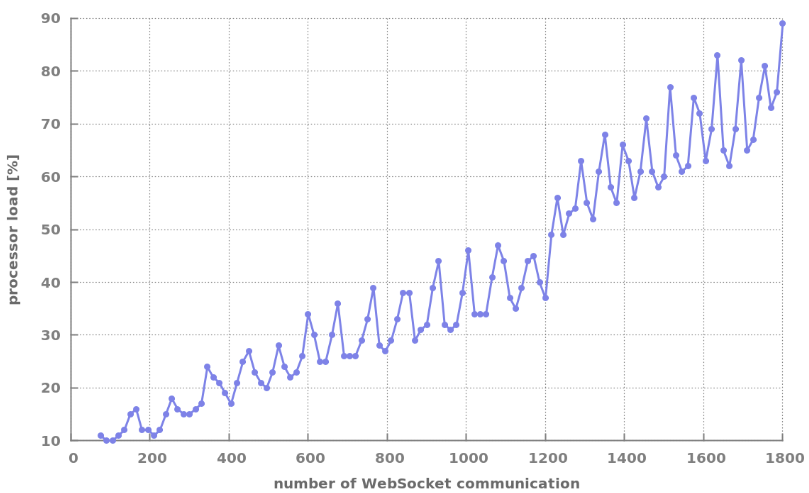
\includegraphics[width=0.9\textwidth]{./Figures/1_client.png}
	\caption[1_client]{One client throughout}
	\label{fig:1_client}
\end{figure}

\begin{figure}[H]
	\centering
		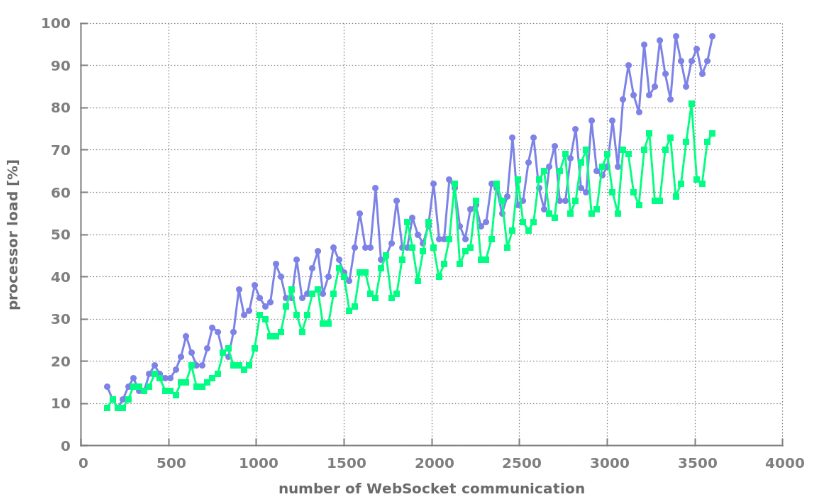
\includegraphics[width=0.9\textwidth]{./Figures/2_client.png}
	\caption[2_client]{Two clients throughout}
	\label{fig:2_client}
\end{figure}

From \ref{fig:1_client} and  \ref{fig:2_client} can be inferred that the client implementation works flawlessly. Adding a second core enables twice as much communication  to be established.

\subsection{Client browser}

Browsers can be configured to connect to one of the SocketCluster worker. For example if the experiment is run locally, typing \texttt{localhost:8080} in the url will make the browser listen to the port 8080. After what sending ping thanks to \texttt{socket.emit('ping')} can help to check the throughout performance. It also displays the growing number of pings a working has sent since begenning of the experiment.

INSERT GRAPH

\section{Server side}
